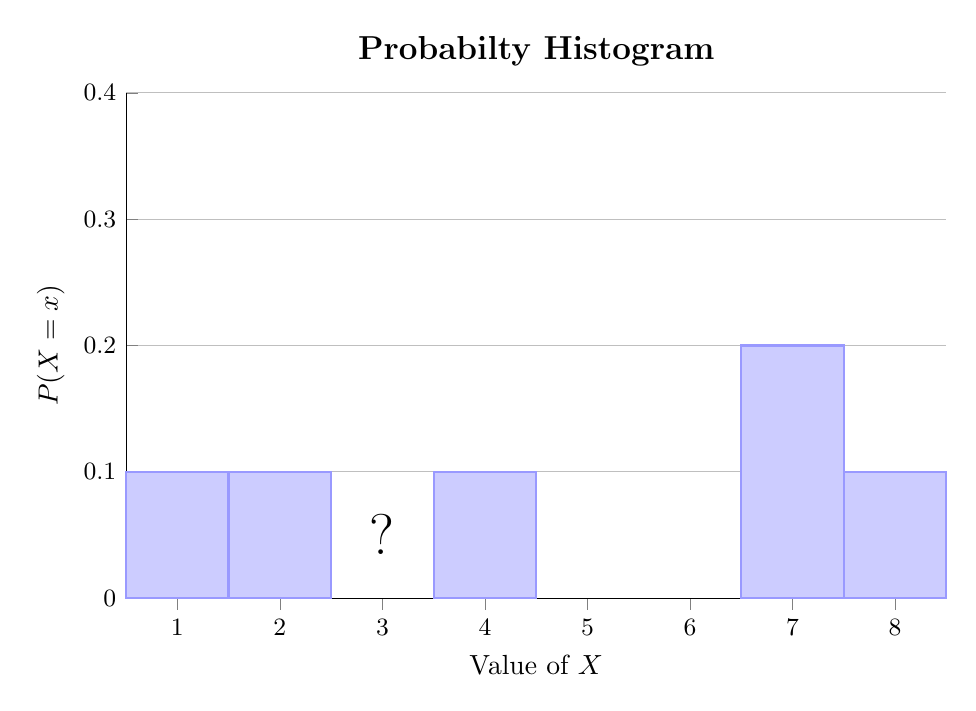
\begin{tikzpicture}
  \begin{axis}[
      axis lines*=left,
      no markers,
      xmin=0.5, xmax=8.5, ymin=0, ymax=0.4,
      xtick={0,1,...,8},
      ytick={0,0.1,0.2,0.3,0.4},
      xlabel={Value of $X$},
      ylabel={$P(X=x)$},
      title={\large\bf Probabilty Histogram},
      ticklabel style={font=\small},
      enlargelimits=false,
      clip=false,
      grid = none,
      ymajorgrids=true,
      ybar=0pt,
      bar width=1,
      width=12cm,
      height=8cm
    ]
    \addplot+[thick,fill=blue!20,draw=blue!40]  coordinates { 
      (1,0.1)
      (2,0.1)
      (4,0.1)
      (7,0.2)
      (8,0.1)
    };
    \node at (axis cs: 3,0.05) {\huge ?};
  \end{axis}
\end{tikzpicture}
